\chap{Buttons/Switches}


\section{Objectives}
In this lab, you will
\begin{itemize}
    \item Learn how to add new C source files and C header files in an STM32 project, 
    \item Learn how to read digital inputs and display values to LEDs using a timer interrupt of a microcontroller (MCU). 
    \item Learn how to debounce when reading a button.
    \item Learn how to create an FSM and implement an FSM in an MCU.
\end{itemize}

\section{Introduction}
Embedded systems usually use buttons (or keys, or switches, or any form of mechanical contacts) as part of their user interface. This general rule applies from the most basic remote-control system for opening a garage door, right up to the most sophisticated aircraft autopilot system. Whatever the system you create, you need to be able to create a reliable button interface. 

%add a picture of buttons/switch

A button is generally hooked up to an MCU so as to generate a certain logic level when pushed or closed or ``active" and the opposite logic level when unpushed or open or ``inactive."  The active logic level can be either `0' or `1', but for reasons both historical and electrical, an active level of '0' is more common.

We can use a button if we want to perform operations such as:
\begin{itemize}
    \item Drive a motor while a switch is pressed.
    \item Switch on a light while a switch is pressed.
    \item Activate a pump while a switch is pressed.
\end{itemize}
These operations could be implemented using an electrical button without using an MCU; however, use of an MCU may well be appropriate if we require more complex behaviours. For example:
\begin{itemize}
    \item Drive a motor while a switch is pressed. 
    
    \textbf{Condition}: If the safety guard is not in place, don't turn the motor. Instead sound a buzzer for 2 seconds. 
    \item Switch on a light while a switch is pressed.
    
    \textbf{Condition}: To save power, ignore requests to turn on the light during daylight hours. 
    
    \item Activate a pump while a switch is pressed
    
    \textbf{Condition}: If the main water reservoir is below 300 litres, do not start the main pump: instead, start the reserve pump and draw the water from the emergency tank. 
\end{itemize}

In this lab, we consider how you read inputs from mechanical buttons in your embedded application using an MCU. 

% Before considering button/switches themselves, we will consider the process of reading the state of port pins.
\newpage
\section{Basic techniques for reading from port pins}
\subsection{The need for pull-up resistors}
\begin{figure}[!htp]
    \centering
    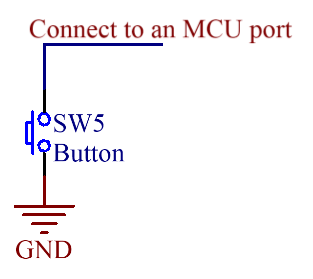
\includegraphics[width=2in]{source/picture/bai_3/Button_Schematic_0.png}
    \caption{\textit{Connecting a button to an MCU}}
    \label{bai4_pic_button_schematic_0}
\end{figure}
Figure \ref{bai4_pic_button_schematic_0} shows a way to connect a button to an MCU. This hardware operates as follows:
\begin{itemize}
    \item When the switch is open, it has no impact on the port pin. An internal resistor on the port ``pulls up" the pin to the supply voltage of the MCU (typically 3.3V for STM32F103). If we read the pin, we will see the value `1'. 
    \item When the switch is closed (pressed), the pin voltage will be 0V. If we read the pin, we will see the value `0'. 
\end{itemize}
 
 However, if the MCU does not have a pull-up resistor inside, when the button is pressed, the read value will be `0', but even we release the button, the read value is still `0' as shown in Figure \ref{bai4_pic_the_need_of_pull_up_resistors}.
 \begin{figure}[!htp]
    \centering
    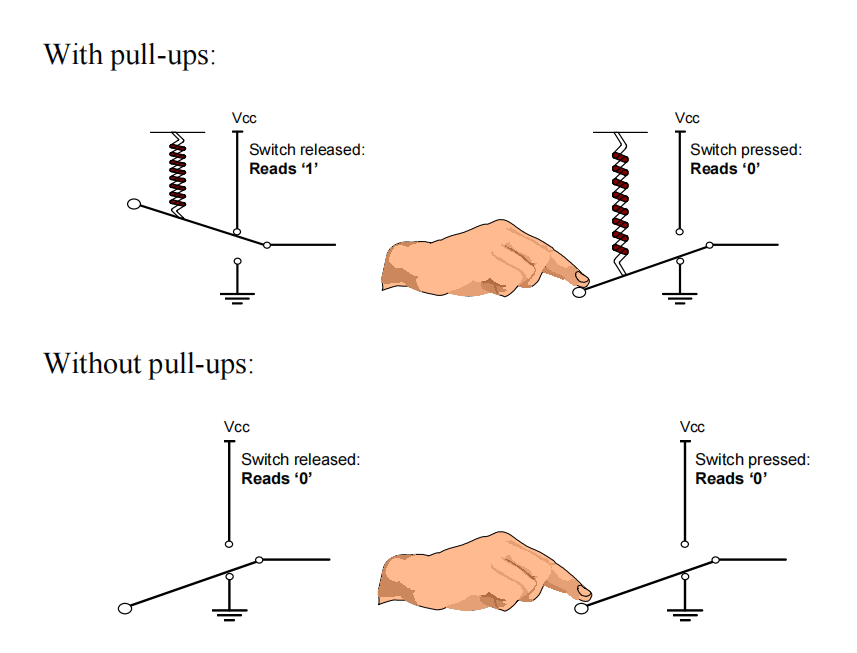
\includegraphics[width=4.5in]{source/picture/bai_3/pullup_resistors.png}
    \caption{\textit{The need of pull up resistors}}
    \label{bai4_pic_the_need_of_pull_up_resistors}
\end{figure}
%add a picture 

So a reliable way to connect a button/switch to an MCU is that we explicitly use an external pull-up resistor as shown in Figure \ref{bai4_pic_button_schematic_1}.

 \begin{figure}[!htp]
    \centering
    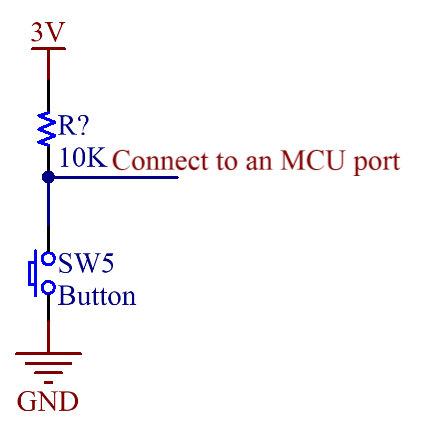
\includegraphics[width=2in]{source/picture/bai_3/Button_Schematic.png}
    \caption{\textit{A reliable way to connect a button to an MCU}}
    \label{bai4_pic_button_schematic_1}
\end{figure}
 
%\newpage 
\subsection{Dealing with switch bounces}
In practice, all mechanical switch contacts bounce (that is, turn on and off, repeatedly, for short period of time) after the switch is closed or opened as shown in Figure \ref{bai4_pic_switchsbounce}.
\begin{figure}[!htp]
    \centering
    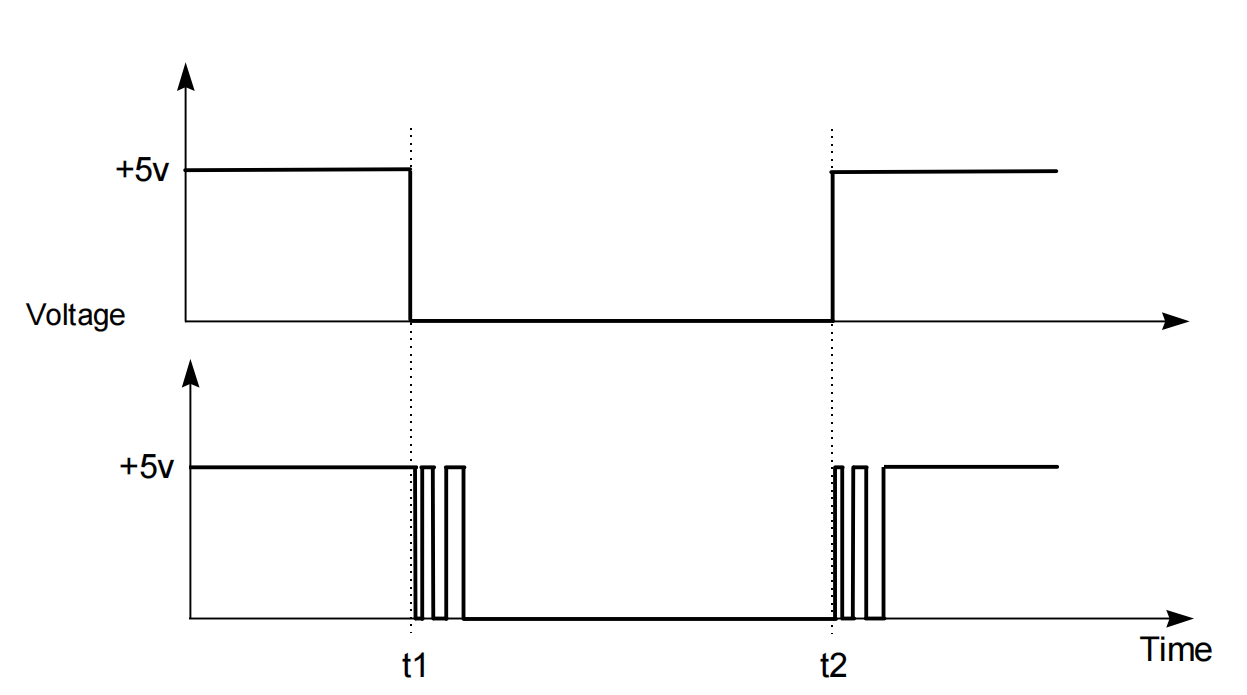
\includegraphics[width=4.5in]{source/picture/bai_3/switchsbounce.png}
    \caption{\textit{Switch bounces}}
    \label{bai4_pic_switchsbounce}
\end{figure}

Every system that uses any kind of mechanical switch must deal with the issue of debouncing.  The key task is to make sure that one mechanical switch or button action is only read as one action by the MCU, even though the MCU will typically be fast enough to detect the unwanted switch bounces and treat them as separate events.  Bouncing can be eliminated by special ICs or by RC circuitry, but in most cases debouncing is done in software because software is ``free".

As far as the MCU concerns, each ``bounce" is equivalent to one press and release of an ``ideal” switch. 
Without appropriate software design, this can give several problems:
\begin{itemize}
    \item Rather than reading ‘A’ from a keypad, we may read ‘AAAAA’
    \item Counting the number of times that a switch is pressed becomes extremely difficult
    \item If a switch is depressed once, and then released some time later, the `bounce' may make it appear as if the switch has been pressed again (at the time of release). 
\end{itemize}


The key to debouncing is to establish a minimum criterion for a valid button push, one that can be implemented in software.  This criterion must involve differences in time - two button presses in 20ms must be treated as one button event, while two button presses in 2 seconds must be treated as two button events.  So what are the relevant times we need to consider?  They are these:
\begin{itemize}
    \item Bounce time:  most buttons seem to stop bouncing within 10ms
    \item Button press time: the shortest time a user can press and release a button seems to be between 50 and 100ms
    \item Response time: a user notices if the system response is 100ms after the button press, but not if it is 50ms after
\end{itemize}



Combining all of these times, we can set a few goals
\begin{itemize}
    \item Ignore all bouncing within 10ms
    \item Provide a response within 50ms of detecting a button push (or release)
    \item Be able to detect a 50ms push and a 50ms release    
\end{itemize}


The simplest debouncing method is to examine the keys (or buttons or switches) every N milliseconds, where N > 10ms (our specified button bounce upper limit) and N <= 50ms (our specified response time).   We then have three possible outcomes every time we read a button:
\begin{itemize}
    \item We read the button in the solid `0' state
    \item We read the button in the solid `1' state
    \item We read the button while it is bouncing (so we will get either a `0' or a `1')
\end{itemize}

Outcomes 1 and 2 pose no problems, as they are what we would always like to happen.  Outcome 3 also poses no problem because during a bounce either state is acceptable.  If we have just pressed an active-low button and we read a '1' as it bounces, the next time through we are guaranteed to read a '0' (remember, the next time through all bouncing will have ceased), so we will just detect the button push a bit later.  Otherwise, if we read a '0' as the button bounces, it will still be '0' the next time after all bouncing has stopped, so we are just detecting the button push a bit earlier.  The same applies to releasing a button.  Reading a single bounce (with all bouncing over by the time of the next read) will never give us an invalid button state.  It's only reading multiple bounces (multiple reads while bouncing is occurring) that can give invalid button states such as repeated push signals from one physical push. 

So if we guarantee that all bouncing is done by the time we next read the button, we're good.  Well, almost good, if we're lucky...

MCUs often live among high-energy beasts, and often control the beasts.  High energy devices make electrical noise, sometimes great amounts of electrical noise.  This noise can, at the worst possible moment, get into your delicate button-and-high-value-pullup circuit and act like a real button push.  Oops, missile launched, sorry!

If the noise is too intense we cannot filter it out using only software, but will need hardware of some sort (or even a redesign).  But if the noise is only occasional, we can filter it out in software without too much bother.  The trick is that instead of regarding a single button `make' or `break' as valid, we insist on N contiguous makes or breaks to mark a valid button event.  N will be a factor of your button scanning rate and the amount of filtering you want to add.  Bigger N gives more filtering.  The simplest filter (but still a big improvement over no filtering) is just an N of 2, which means compare the current button state with the last button state, and only if both are the same is the output valid.

Note that now we have not two but three button states: active (or pressed), inactive (or released), and indeterminate or invalid (in the middle of filtering, not yet filtered).  In most cases we can treat the invalid state the same as the inactive state, since we care in most cases only about when we go active (from whatever state) and when we cease being active (to inactive or invalid).  With that simplification we can look at simple \mathbf{N = 2} filtering reading a button wired to STM32 MCU:
\begin{lstlisting}[caption=Read port pin and deboucing]
void button_reading(void){
    static unsigned char last_button;
    unsigned char raw_button;
    unsigned char filtered_button;
    last_button = raw_button;
    raw_button = HAL_GPIO_ReadPin(BUTTON_1_GPIO_Port, BUTTON_1_Pin);
    if(last_button == raw_button){
        filtered_button = raw_button;
    }
}
\end{lstlisting}

The function button\_reading() must be called no more often than our debounce time (10ms).

To expand to greater filtering (larger N), keep in mind that the filtering technique essentially involves reading the current button state and then either counting or reseting the counter.  We count if the current button state is the same as the last button state, and if our count reaches N we then report a valid new button state.  We reset the counter if the current button state is different than the last button state, and we then save the current button state as the new button state to compare against the next time.  Also note that the larger our value of N the more often our filtering routine must be called, so that we get a filtered response within our specified 50ms deadline.  So for example with an N of 8 we should be calling our filtering routine every 2 - 5ms, giving a response time of 16 - 40ms (>10ms and <50ms).
% Creating a simple software to check for a valid switch input is straightforward:
% \begin{itemize}
%     \item Read the relevant port pin
%     \item If we think we have detected a switch depression, we wait for 50ms and then read the pin again.
%     \item If the second reading confirms the first reading, we assume the switch really has been depressed.
% \end{itemize}

% Note that the figure of ‘50ms’ will depend on the switch used and the deployed environment. 

\newpage
\section{Reading switch input (basic code) using STM32}


To demonstrate the use of buttons/switches in STM32, we use an example which requires to write a program that 
\begin{itemize}
    \item Has a timer which has an interrupt in every 10 milliseconds.  
    \item Reads values of button PB0 every 10 milliseconds. 
    \item Increases the value of LEDs connected to PORTA by one unit when the button PB0 is pressed.
    \item Increases the value of PORTA automatically in every 0.5 second, if the button PB0 is pressed in more than 1 second.

\end{itemize}
\subsection{Input Output Processing Patterns}
For both input and output processing, we have a similar pattern to work with. Normally, we have a module named driver which works directly to the hardware. We also have a buffer to store temporarily values. In the case of input processing, the driver will store the value of the hardware status to the buffer for further processing. In the case of output processing, the driver uses the buffer data to output to the hardware. 

\begin{figure}[!htp]
    \centering
    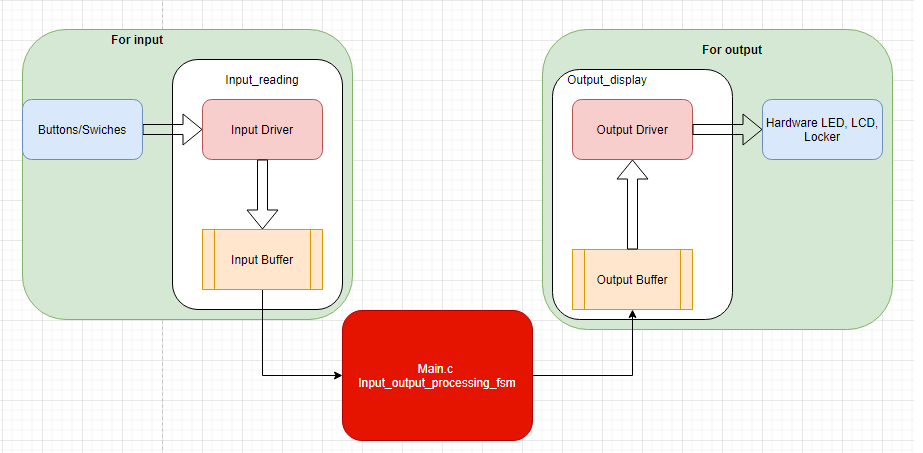
\includegraphics[width=5.5in]{source/picture/bai_3/Input_Output_patterns.png}
    \caption{\textit{Input Output Processing Patterns}}
    \label{bai4_pic_Input_Output_patterns}
\end{figure}

Figure \ref{bai4_pic_Input_Output_patterns} shows that we should have an \emph{input\_reading} module to processing the buttons, then store the processed data to the buffer. Then a module of \emph{input\_output\_processing\_fsm} will process the input data, and update the output buffer. The output driver gets the value from the output buffer to transfer to the hardware. 
\newpage
\subsection{Setting up}
\subsubsection{Create a project}
Please follow the instruction in Labs 1 and 2 to create a project that includes: 
\begin{itemize}
    \item PB0 as an input port pin, 
    \item PA0-PA7 as output port pins, and 
    \item Timer 2 10ms interrupt
\end{itemize}

% \begin{figure}[!htp]
%     \centering
%     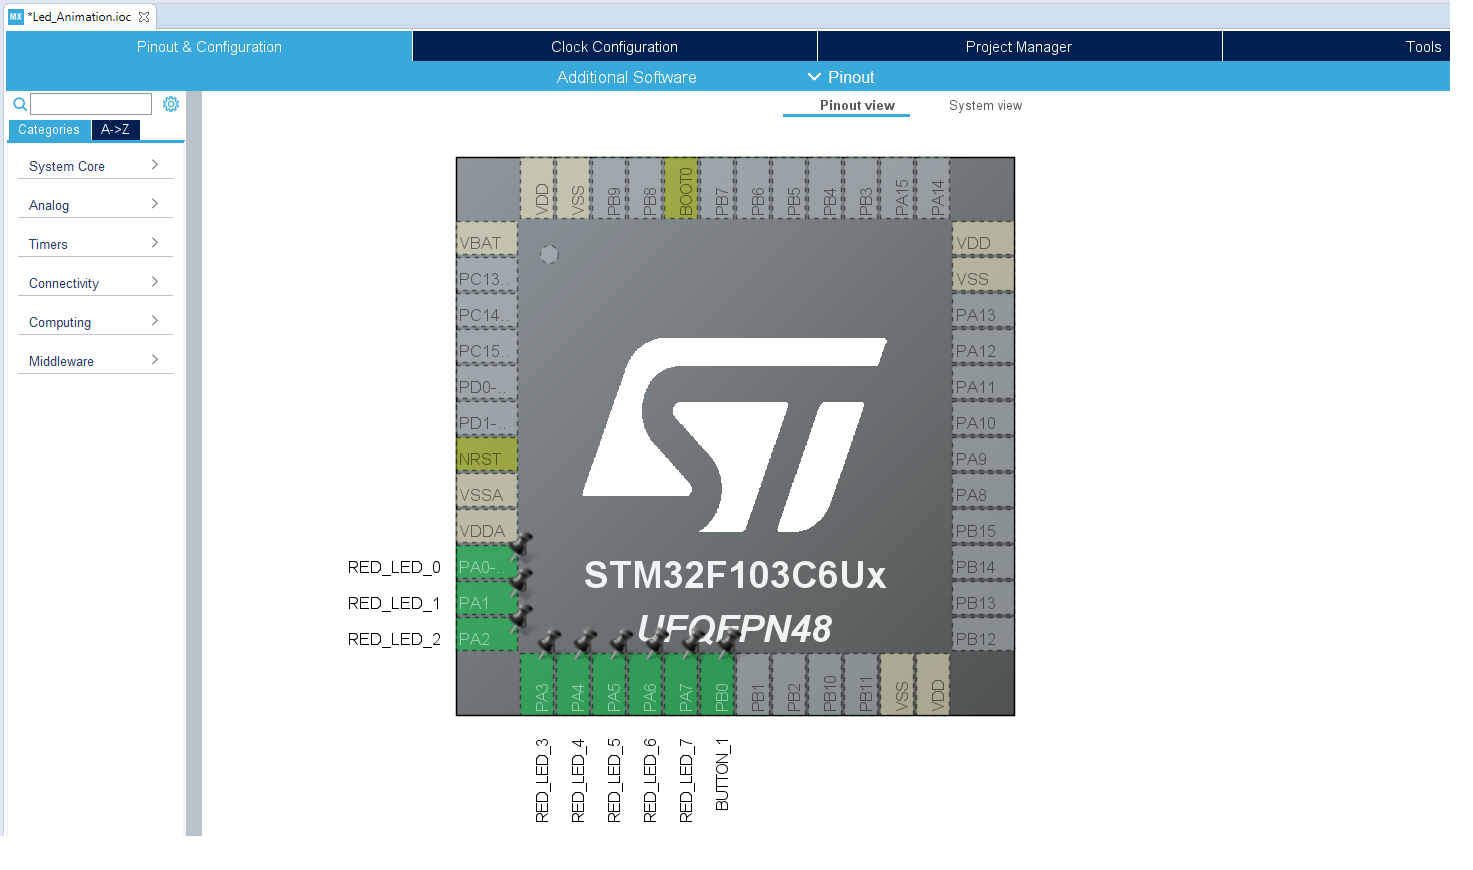
\includegraphics[width=5.5in]{source/picture/bai_3/Input_Output_Settings.png}
%     \caption{\textit{Input Output Setting}}
%     \label{bai4_pic_input_output_setting}
% \end{figure}


\subsubsection{Create a file C source file and header file for input reading}
We are expected to have files for button processing and led display as shown in Figure \ref{bai4_pic_Adding_new_files_to_project}.

\begin{figure}[!htp]
    \centering
    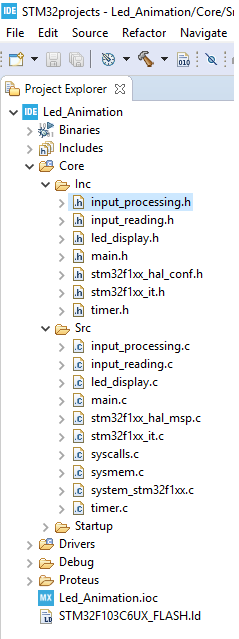
\includegraphics[width=1.5in]{source/picture/bai_3/Adding_new_files_to_project.png}
    \caption{\textit{File Organization}}
    \label{bai4_pic_Adding_new_files_to_project}
\end{figure}

Steps 1 (Figure \ref{bai4_pic_Adding_new_files_to_project_step_1}): Right click to the folder \textbf{Src}, select \textbf{New}, then select \textbf{Source File}. There will be a pop-up. Please type the file name, then click \textbf{Finish}.
\begin{figure}[!htp]
    \centering
    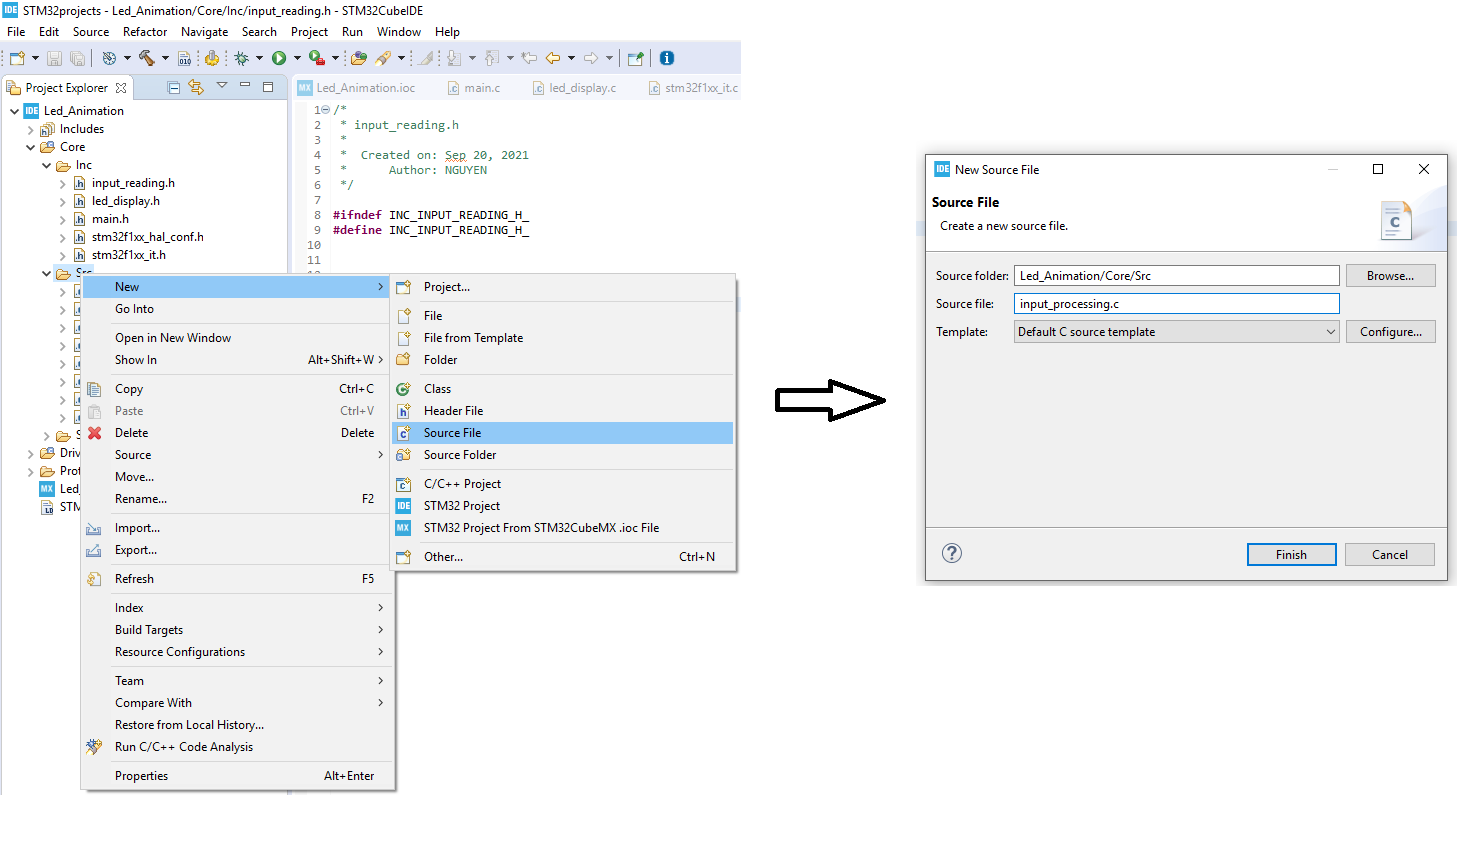
\includegraphics[width=5.5in]{source/picture/bai_3/Adding_new_files_to_project_step_1.png}
    \caption{\textit{Step 1: Create a C source file for input reading}}
    \label{bai4_pic_Adding_new_files_to_project_step_1}
\end{figure}

Step 2 (Figure \ref{bai4_pic_Adding_new_files_to_project_step_3}): Do the same for the C header file in the folder \textbf{Inc}.
\begin{figure}[!htp]
    \centering
    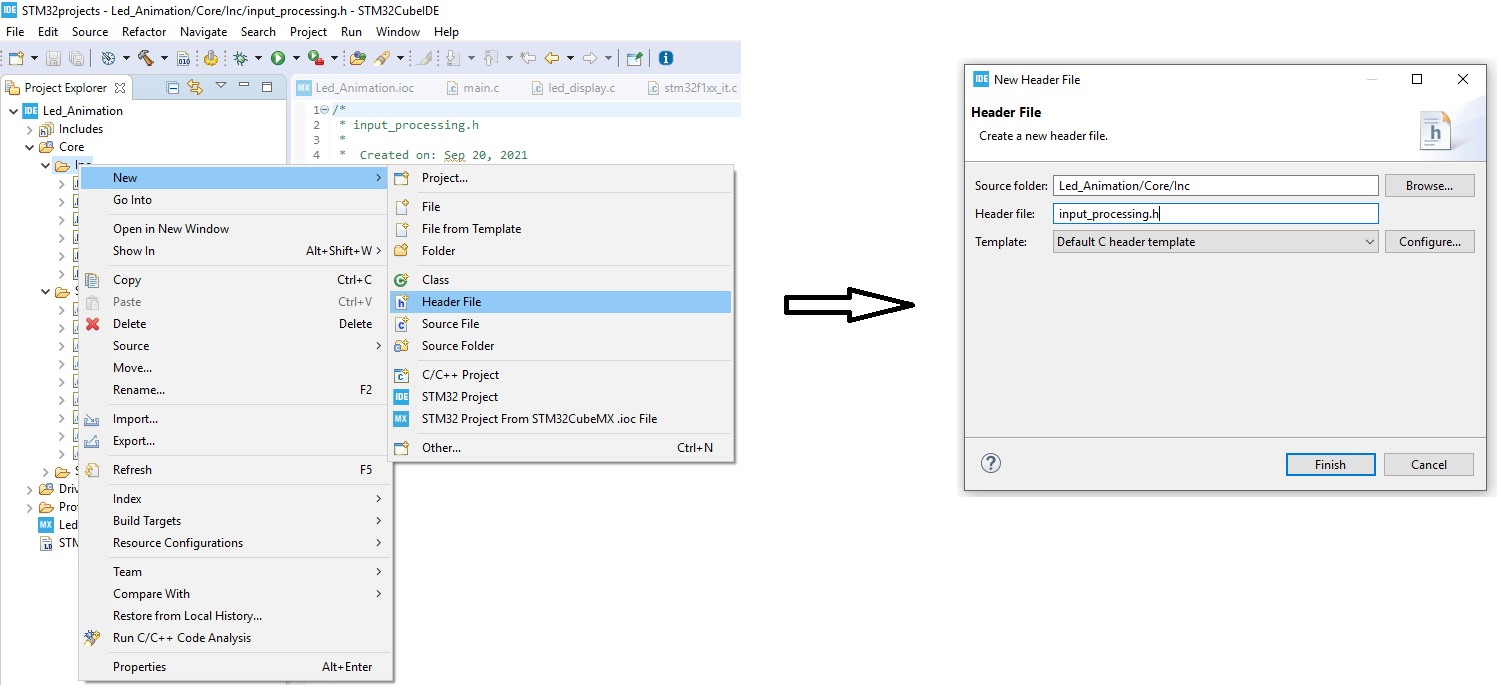
\includegraphics[width=5.5in]{source/picture/bai_3/Adding_new_files_to_project_step_3.png}
    \caption{\textit{Step 2: Create a C header file for input processing}}
    \label{bai4_pic_Adding_new_files_to_project_step_3}
\end{figure}


\newpage

\newpage
\subsection{Code For Read Port Pin and Debouncing}
\subsubsection{The code in the input\_reading.c file}
\begin{lstlisting}[caption=Define constants buffers and button\_reading function]
#include "main.h"
//we aim to work with more than one buttons
#define N0_OF_BUTTONS 				       1
//timer interrupt duration is 10ms, so to pass 1 second, 
//we need to jump to the interrupt service routine 100 time
#define DURATION_FOR_AUTO_INCREASING	   100
#define BUTTON_IS_PRESSED                  GPIO_PIN_RESET
#define BUTTON_IS_RELEASED                 GPIO_PIN_SET
//the buffer that the final result is stored after 
//debouncing
static GPIO_PinState buttonBuffer[N0_OF_BUTTONS];
//we define two buffers for debouncing
static GPIO_PinState debounceButtonBuffer1[N0_OF_BUTTONS];
static GPIO_PinState debounceButtonBuffer2[N0_OF_BUTTONS];
//we define a flag for a button pressed more than 1 second.
static uint8_t flagForButtonPress1s[N0_OF_BUTTONS];
//we define counter for automatically increasing the value 
//after the button is pressed more than 1 second.
static uint16_t counterForButtonPress1s[N0_OF_BUTTONS];
void button_reading(void){
	for(char i = 0; i < N0_OF_BUTTONS; i ++){
		debounceButtonBuffer2[i] =debounceButtonBuffer1[i];
		debounceButtonBuffer1[i] = HAL_GPIO_ReadPin(BUTTON_1_GPIO_Port, BUTTON_1_Pin);
		if(debounceButtonBuffer1[i] == debounceButtonBuffer2[i])
			buttonBuffer[i] = debounceButtonBuffer1[i];
			if(buttonBuffer[i] == BUTTON_IS_PRESSED){
			//if a button is pressed, we start counting
				if(counterForButtonPress1s[i] < DURATION_FOR_AUTO_INCREASING){
					counterForButtonPress1s[i]++;
				} else {
				//the flag is turned on when 1 second has passed 
				//since the button is pressed.
					flagForButtonPress1s[i] = 1;
					//todo
				}
			} else {
				counterForButtonPress1s[i] = 0;
				flagForButtonPress1s[i] = 0;
			}
	}
}
\end{lstlisting}

% The program reads all buttons two consecutive times and compare the values. If the values are the same, update the value to buttonBuffer. This function should be called inside the timer interrupt service routine.
% \begin{lstlisting}[caption=Read port pin and deboucing]
% void button_reading(void){
% 	for(char i = 0; i < N0_OF_BUTTONS; i ++){
% 		debounceButtonBuffer2[i] =debounceButtonBuffer1[i];
% 		debounceButtonBuffer1[i] = HAL_GPIO_ReadPin(BUTTON_1_GPIO_Port, BUTTON_1_Pin);
% 		if(debounceButtonBuffer1[i] == debounceButtonBuffer2[i])
% 			buttonBuffer[i] = debounceButtonBuffer1[i];
% 			if(buttonBuffer[i] == BUTTON_IS_PRESSED){
% 			//if a button is pressed, we start counting
% 				if(counterForButtonPress1s[i] < DURATION_FOR_AUTO_INCREASING){
% 					counterForButtonPress1s[i]++;
% 				} else {
% 				//the flag is turned on when 1 second has passed 
% 				//since the button is pressed.
% 					flagForButtonPress1s[i] = 1;
% 					//todo
% 				}

% 			} else {
% 				counterForButtonPress1s[i] = 0;
% 				flagForButtonPress1s[i] = 0;
% 			}
% 	}
% }
% \end{lstlisting}


\begin{lstlisting}[caption=Checking a button is pressed or not]
unsigned char is_button_pressed(uint8_t index){
	if(index >= N0_OF_BUTTONS) return 0;
	return (buttonBuffer[index] == BUTTON_IS_PRESSED);
}
\end{lstlisting}
\begin{lstlisting}[caption=Checking a button is pressed more than a second or not]
unsigned char is_button_pressed_1s(unsigned char index){
	if(index >= N0_OF_BUTTONS) return 0xff;
	return (flagForButtonPress1s[index] == 1);
}
\end{lstlisting}
\subsubsection{The code in the input\_reading.h file}
\begin{lstlisting}[caption=Prototype in input\_reading.h file]
#ifndef INC_INPUT_READING_H_
#define INC_INPUT_READING_H_
void button_reading(void);
unsigned char is_button_pressed(unsigned char index);
unsigned char is_button_pressed_1s(unsigned char index);
#endif /* INC_INPUT_READING_H_ */
\end{lstlisting}

\subsubsection{The code in the timer.c file}
\begin{lstlisting}[caption=Timer interrupt callback function]
#include "main.h"
#include "input_reading.h"

void HAL_TIM_PeriodElapsedCallback(TIM_HandleTypeDef *htim)
{
	if(htim->Instance == TIM2){
		button_reading();
	}
}

\end{lstlisting}



\newpage
\subsection{Button State Processing}
\subsubsection {Finite State Machine}
To solve the example problem, we define 3 states as follows:
\begin{itemize}
    \item State 0: The button is released or the button is in the initial state. 
    \item State 1: When the button is pressed, the FSM will change to State 1 that is increasing the values of PORTA by one value. If the button is released, the FSM goes back to State 0.
    \item State 2: while the FSM is in State 1, the button is kept pressing more than 1 second, the state of FSM will change from 1 to 2. In this state, if the button is kept pressing, the value of PORTA will be increased automatically in every 500ms. If the button is released, the FSM goes back to State 0.
\end{itemize}
\begin{figure}[!htp]
    \centering
    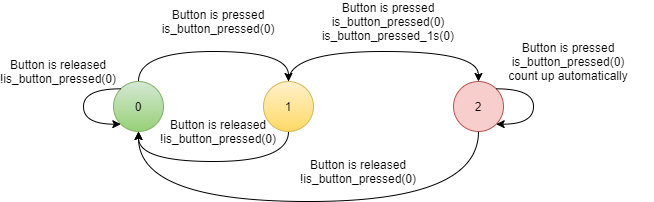
\includegraphics[width=5.5in]{source/picture/bai_3/fsm.png}
    \caption{\textit{An FSM for processing a button}}
    \label{bai4_pic_fsm_for_button_processing}
\end{figure}
\newpage
\subsubsection{The code for the FSM in the input\_processing.c file}
Please note that \emph{fsm\_for\_input\_processing} function should be called inside the super loop of the main functin. 
\begin{lstlisting}[caption=The code in the input\_processing.c file]
#include "main.h"
#include "input_reading.h"

enum ButtonState{BUTTON_RELEASED, BUTTON_PRESSED, BUTTON_PRESSED_MORE_THAN_1_SECOND} ;
enum ButtonState buttonState = BUTTON_RELEASED;
void fsm_for_input_processing(void){
	switch(buttonState){
	case BUTTON_RELEASED:
		if(is_button_pressed(0)){
			buttonState = BUTTON_PRESSED;
			//INCREASE VALUE OF PORT A BY ONE UNIT
		}
		break;
	case BUTTON_PRESSED:
		if(!is_button_pressed(0)){
			buttonState = BUTTON_RELEASED;
		} else {
			if(is_button_pressed_1s(0)){
				buttonState = BUTTON_PRESSED_MORE_THAN_1_SECOND;
			}
		}
		break;
	case BUTTON_PRESSED_MORE_THAN_1_SECOND:
		if(!is_button_pressed(0)){
			buttonState = BUTTON_RELEASED;
		}
		//todo
		break;
	}
}
\end{lstlisting}
\subsubsection{The code in the input\_processing.h}
\begin{lstlisting}[caption=Code in the input\_processing.h file]
#ifndef INC_INPUT_PROCESSING_H_
#define INC_INPUT_PROCESSING_H_

void fsm_for_input_processing(void);

#endif /* INC_INPUT_PROCESSING_H_ */
\end{lstlisting}


\subsubsection{The code in the main.c file}
\begin{lstlisting}[caption=The code in the main.c file]
#include "main.h"
#include "input_processing.h"
//don't modify this part
int main(void){
    HAL_Init();
    /* Configure the system clock */
    SystemClock_Config();
    /* Initialize all configured peripherals */
    MX_GPIO_Init();
    MX_TIM2_Init();
    while (1)
    {
        //you only need to add the fsm function here
        fsm_for_input_processing();
    }
}
\end{lstlisting}

\newpage
\section{Exercises and Report}
\subsection{Specifications}
You are required to build an application of a traffic light in a cross road which includes some features as described below:
\begin{itemize}
    \item The application has 12 LEDs including 4 red LEDs, 4 amber LEDs, 4 green LEDs.
    \item The application has 4 seven segment LEDs to display time with 2 for each road. The 2 seven segment LEDs will show time for each color LED corresponding to each road.
    \item The application has three buttons which are used
    \subitem - to select modes, 
    \subitem - to modify the time for each color led on the fly, and 
    \subitem - to set the chosen value. 
    \item The application has at least 4 modes which is controlled by the first button. Mode 1 is a normal mode, while modes 2 3 4 are  modification modes. You can press the first button to change the mode. Modes will change from 1 to 4 and back to 1 again. 
    
    \textbf{Mode 1 - Normal mode}: 
    \subitem - The traffic light application is running normally.   
    
    \textbf{Mode 2 - Modify time duration for the red LEDs}: This mode allows you to change the time duration of the red LED in the main road. The expected behaviours of this mode include:  
    \subitem - All single red LEDs are blinking in 2 Hz. 
    \subitem - Use two seven-segment LEDs to display the value.
    \subitem - Use the other two seven-segment LEDs to display the mode.
    \subitem - The second button is used to increase the time duration value for the red LEDs. 
    \subitem - The value of time duration is in a range of 1 - 99. 
    \subitem - The third button is used to set the value.
    
    
    \textbf{Mode 3 - Modify time duration for the amber LEDs}: Similar for the red LEDs described above with the amber LEDs.
    
    
    \textbf{Mode 4 - Modify time duration for the green LEDs}: Similar for the red LEDs described above with the green LEDs.
\end{itemize}

\newpage
\subsection{Exercise 1: Sketch an FSM}
Your task in this exercise is to sketch an FSM that describes your idea of how to solve the problem.

Please add your report here.

\subsection{Exercise 2: Proteus Schematic}
Your task in this exercise is to draw a Proteus schematic for the problem above. 

Please add your report here.


\subsection{Exercise 3: Create STM32 Project}
Your task in this exercise is to create a project that has pin corresponding to the Proteus schematic that you draw in previous section. You need to set up your timer interrupt is about 10ms.

Please add your report here.

\subsection{Exercise 4: Modify Timer Parameters}
Your task in this exercise is to modify the timer settings so that when we want to change the time duration of the timer interrupt, we change it the least and it will not affect the overall system. For example, the current system we have implemented is that it can blink an LED in 2 Hz, with the timer interrupt duration is 10ms. However, when we want to change the timer interrupt duration to 1ms or 100ms, it will not affect the 2Hz blinking LED. 

Please add your report here.
\subsection{Exercise 5: Adding code for button debouncing}
Following the example of button reading and debouncing in the previous section, your tasks in this exercise are:
\begin{itemize}
    \item To add new files for input reading and output display,
    \item To add code for button debouncing,
    \item To add code for increasing mode when the first button is pressed. 
\end{itemize}

Please add your report here.
\newpage
\subsection{Exercise 6: Adding code for displaying modes}
Your tasks in this exercise are:
\begin{itemize}
    \item To add code for display mode on seven-segment LEDs, and
    \item To add code for blinking LEDs depending on the mode that is selected. 
\end{itemize}

Please add your report here.
\subsection{Exercise 7: Adding code for increasing time duration value for the red LEDs}
Your tasks in this exercise are: 
\begin{itemize}
    \item to use the second button to increase the time duration value of  the red LEDs
    \item to use the third button to set the value for the red LEDs.
\end{itemize}
Please add your report here.

\subsection{Exercise 8: Adding code for increasing time duration value for the amber LEDs}

Your tasks in this exercise are: 
\begin{itemize}
    \item to use the second button to increase the time duration value of the amber LEDs
    \item to use the third button to set the value for the amber LEDs.
\end{itemize}
Please add your report here.
\subsection{Exercise 9: Adding code for increasing time duration value for the green LEDs}

Your tasks in this exercise are: 
\begin{itemize}
    \item to use the second button to increase the  time duration value of the green LEDs
    \item to use the third button to set the value for the green LEDs.
\end{itemize}
Please add your report here.

\subsection{Exercise 10: To finish the project}
Your tasks in this exercise are:
\begin{itemize}
    \item To integrate all the previous tasks to one final project
    \item To create a video to show all features in the specification
    \item To add a report to describe your solution for each exercise.
    \item To submit your report and code on the BKeL
\end{itemize}

% \section{Problem 1}

% In this week lab, assume you have two button and 8 LEDs, you have to write a program that
% \begin{itemize}
%     \item Has a timer which has an interrupt in every 10 milliseconds.  
%     \item  Reads values of buttons 1 and 2 every 10 milliseconds. The read button function should be called inside the timer interrupt service routine.
%     \item Increases the value of LEDs connected to PORTA when the button 1 is pressed.
%     \item Increases the value of PORTA automatically in every 0.5 second, if the button 1 is pressed in more than 1 second.
%     \item Increases the value of PORTA automatically in every 0.1 second, if the button 1 is pressed in more than 3 seconds.
%     \item Decreases the value of PORTA when the button 2 is pressed
%     \item Decreases the value of PORTA automatically in every 0.5 second, if the button 2 is pressed in more than 1 second.
%     \item Decreases the value of PORTA automatically in every 0.1 second, if the button 2 is pressed in more than 3 seconds.
%     \item The above values such as 10 ms, 0.5 s, 0.1s, 1 s and 3 s are fixed values as an example. Your program, however, needs to provide an easy way to change those values. For example, you should use DEFINE to define those values.
%     \item If both buttons 1 and 2 are pressed, button 1 has a higher priority.
% \end{itemize}


% \section{Problem 2 - A digital clock}
%  You have to write a program that mimics a Casio digital watch. Assume you have 2 buttons and 6 seven-segment LED, a program should have
% \begin{itemize}
%     \item A normal clock that shows hours, minutes, and seconds on 6 seven-segment LEDs.
%     \item  A stopwatch that shows minutes, seconds and 1/100 second
%     \item We use button 1 to change modes of a digital watch. Every time button 1 is pressed, the watch will change to the next mode.
%     \item Mode 0: runs normal clock (default)
%     \item Mode 1: modifies hours. In this mode, the hour number is blinking, and button 2 is used for increasing the hour number.  If button 2 is kept pressed more than 1 second, the hour number will increase automatically, i.e., 5 times per second. Please note that the hour number should be returned to 0 when it reaches 23.
%     \item  Mode 2: modifies minutes. Similar to mode 1, the minute number is blinking and increases when button 2 is pressed.
%     \item Mode 3: modifies seconds. Similar to mode 1, the second number is blinking and increases when button 2 is pressed.
%     \item Mode 4: runs a stopwatch. Using button 2 to start and stop the watch.  
 
% \end{itemize}
%  Please note that while the stopwatch is running, the normal clock is still running in the background.


 

% \section{Instructions}

% Your task is to sketch an FSM that describes your idea of how to solve the above problems and  writes a firmware that runs on STM32.



 

% \section{Submission}

% You need to
% \begin{itemize}
%     \item Demonstrate your work in the lab class and then
%     \item  Submit your FSM sketches and source code to the BKeL.
% \end{itemize}
